\documentclass[journal,12pt,twocolumn]{IEEEtran}

\usepackage{setspace}
\usepackage{gensymb}
\singlespacing
\usepackage[cmex10]{amsmath}

\usepackage{amsthm}

\usepackage{mathrsfs}
\usepackage{txfonts}
\usepackage{stfloats}
\usepackage{bm}
\usepackage{cite}
\usepackage{cases}
\usepackage{subfig}

\usepackage{longtable}
\usepackage{multirow}

\usepackage{enumitem}
\usepackage{mathtools}
\usepackage{steinmetz}
\usepackage{tikz}
\usepackage{circuitikz}
\usepackage{verbatim}
\usepackage{tfrupee}
\usepackage[breaklinks=true]{hyperref}
\usepackage{graphicx}
\usepackage{tkz-euclide}

\usetikzlibrary{calc,math}
\usepackage{listings}
    \usepackage{color}                                            %%
    \usepackage{array}                                            %%
    \usepackage{longtable}                                        %%
    \usepackage{calc}                                             %%
    \usepackage{multirow}                                         %%
    \usepackage{hhline}                                           %%
    \usepackage{ifthen}                                           %%
    \usepackage{lscape}     
\usepackage{multicol}
\usepackage{chngcntr}

\DeclareMathOperator*{\Res}{Res}

\renewcommand\thesection{\arabic{section}}
\renewcommand\thesubsection{\thesection.\arabic{subsection}}
\renewcommand\thesubsubsection{\thesubsection.\arabic{subsubsection}}

\renewcommand\thesectiondis{\arabic{section}}
\renewcommand\thesubsectiondis{\thesectiondis.\arabic{subsection}}
\renewcommand\thesubsubsectiondis{\thesubsectiondis.\arabic{subsubsection}}


\hyphenation{op-tical net-works semi-conduc-tor}
\def\inputGnumericTable{}                                 %%

\lstset{
%language=C,
frame=single, 
breaklines=true,
columns=fullflexible
}
\begin{document}


\newtheorem{theorem}{Theorem}[section]
\newtheorem{problem}{Problem}
\newtheorem{proposition}{Proposition}[section]
\newtheorem{lemma}{Lemma}[section]
\newtheorem{corollary}[theorem]{Corollary}
\newtheorem{example}{Example}[section]
\newtheorem{definition}[problem]{Definition}

\newcommand{\BEQA}{\begin{eqnarray}}
\newcommand{\EEQA}{\end{eqnarray}}
\newcommand{\define}{\stackrel{\triangle}{=}}
\bibliographystyle{IEEEtran}
\raggedbottom
\setlength{\parindent}{0pt}
\providecommand{\mbf}{\mathbf}
\providecommand{\pr}[1]{\ensuremath{\Pr\left(#1\right)}}
\providecommand{\qfunc}[1]{\ensuremath{Q\left(#1\right)}}
\providecommand{\sbrak}[1]{\ensuremath{{}\left[#1\right]}}
\providecommand{\lsbrak}[1]{\ensuremath{{}\left[#1\right.}}
\providecommand{\rsbrak}[1]{\ensuremath{{}\left.#1\right]}}
\providecommand{\brak}[1]{\ensuremath{\left(#1\right)}}
\providecommand{\lbrak}[1]{\ensuremath{\left(#1\right.}}
\providecommand{\rbrak}[1]{\ensuremath{\left.#1\right)}}
\providecommand{\cbrak}[1]{\ensuremath{\left\{#1\right\}}}
\providecommand{\lcbrak}[1]{\ensuremath{\left\{#1\right.}}
\providecommand{\rcbrak}[1]{\ensuremath{\left.#1\right\}}}
\theoremstyle{remark}
\newtheorem{rem}{Remark}
\newcommand{\sgn}{\mathop{\mathrm{sgn}}}
\providecommand{\abs}[1]{\left\vert#1\right\vert}
\providecommand{\res}[1]{\Res\displaylimits_{#1}} 
\providecommand{\norm}[1]{\left\lVert#1\right\rVert}
%\providecommand{\norm}[1]{\lVert#1\rVert}
\providecommand{\mtx}[1]{\mathbf{#1}}
\providecommand{\mean}[1]{E\left[ #1 \right]}
\providecommand{\fourier}{\overset{\mathcal{F}}{ \rightleftharpoons}}
%\providecommand{\hilbert}{\overset{\mathcal{H}}{ \rightleftharpoons}}
\providecommand{\system}{\overset{\mathcal{H}}{ \longleftrightarrow}}
    %\newcommand{\solution}[2]{\textbf{Solution:}{#1}}
\newcommand{\solution}{\noindent \textbf{Solution: }}
\newcommand{\cosec}{\,\text{cosec}\,}
\providecommand{\dec}[2]{\ensuremath{\overset{#1}{\underset{#2}{\gtrless}}}}
\newcommand{\myvec}[1]{\ensuremath{\begin{pmatrix}#1\end{pmatrix}}}
\newcommand{\mydet}[1]{\ensuremath{\begin{vmatrix}#1\end{vmatrix}}}
\numberwithin{equation}{subsection}
\makeatletter
\@addtoreset{figure}{problem}
\makeatother
\let\StandardTheFigure\thefigure
\let\vec\mathbf
\renewcommand{\thefigure}{\theproblem}
\def\putbox#1#2#3{\makebox[0in][l]{\makebox[#1][l]{}\raisebox{\baselineskip}[0in][0in]{\raisebox{#2}[0in][0in]{#3}}}}
     \def\rightbox#1{\makebox[0in][r]{#1}}
     \def\centbox#1{\makebox[0in]{#1}}
     \def\topbox#1{\raisebox{-\baselineskip}[0in][0in]{#1}}
     \def\midbox#1{\raisebox{-0.5\baselineskip}[0in][0in]{#1}}
\vspace{3cm}
\title{Assignment 1}
\author{ADYASA MOHANTY - EE18BTECH11048}
\maketitle
\newpage
\bigskip
\renewcommand{\thefigure}{\theenumi}
\renewcommand{\thetable}{\theenumi}
Download all python codes from 
\begin{lstlisting}
https://github.com/adyasa611/EE3250/blob/main/Assignment-1/Codes
\end{lstlisting}
%
and latex-tikz codes from 
%
\begin{lstlisting}
https://github.com/adyasa611/EE3250/blob/main/Assignment-1/Figures
\end{lstlisting}
\section{DIGITAL FILTER}
\begin{enumerate}[label=\thesection.\arabic*
,ref=\thesection.\theenumi]
\item
\label{prob:input}
Download the sound file from  
\begin{lstlisting}
https://raw.githubusercontent.com/gadepall/ EE1310/master/filter/codes/Sound_Noise.wav
\end{lstlisting}

\item
\label{prob:output}
Write the python code for removal of out of band noise and execute the code.
\\
\solution
\lstinputlisting{./code/cancel_noise.py}
\end{enumerate}
\section{Difference equation}
\begin{enumerate}[label=\thesection.\arabic*,ref=\thesection.\theenumi]
\item
\label{prob:diff_eq}
Write the difference equation of above Digital filter obtained in problem \ref{prob:output}.
\\
\solution
\begin{equation}
\label{eq:iir_filter_gen}
 \sum _{m=0}^{M}a\brak{m}y\brak{n-m}=\sum _{k=0}^{N}b\brak{k}x\brak{n-k}
\end{equation}
\begin{equation}
\label{eq:diff_eqn}
\begin{split}
y(n) - 2.52y(n-1) + 2.56y(n-2) - 1.206y(n-3)
\\
+ 0.22013y(n-4) = 0.00345x(n) + 0.0138x(n-1) +
\\
 0.020725x(n-2) + 0.0138x(n-3) + 0.00345x(n-4)
\end{split}
\end{equation}

\item
\label{prob:xnyn_plot1}
Sketch x(n) and y(n).
\\
\solution
The following code yields Fig. \ref{fig:xnyn}
\begin{lstlisting}
Codes/plot_xn_yn.py
\end{lstlisting}
The filtered sound signal obtained through difference equation :
\begin{lstlisting}
Codes/Sound_diff_eq.wav
\end{lstlisting}
\begin{figure}[!ht]
\begin{center}
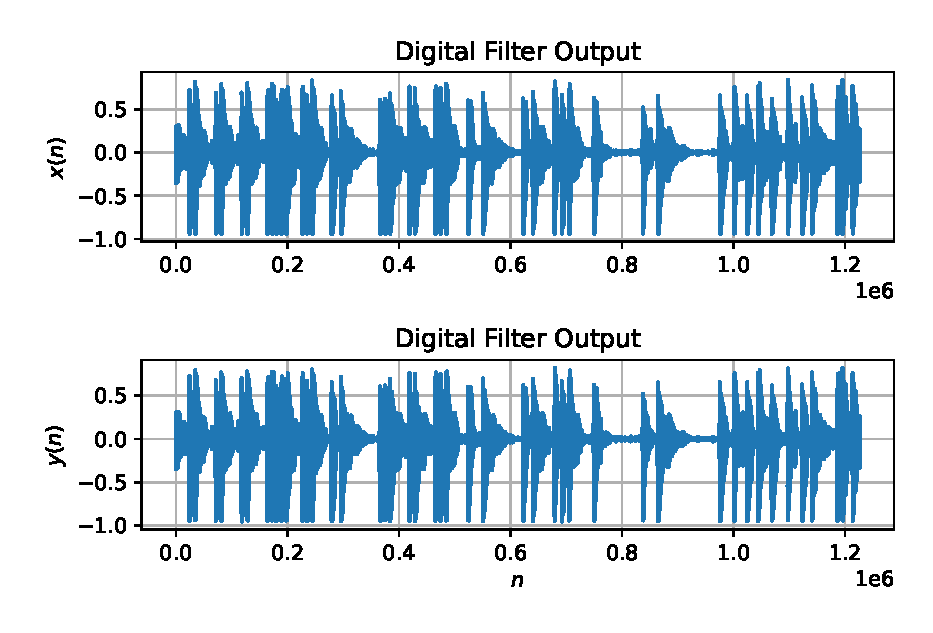
\includegraphics[width=\columnwidth]{xn_yn}
\end{center}
\captionof{figure}{}
\label{fig:xnyn}    
\end{figure}
\end{enumerate}
\section{Z-transform}
\begin{enumerate}[label=\thesection.\arabic*,ref=\thesection.\theenumi]
\item
\label{prob:Z-transform_formula}
%
\begin{equation}
\label{eq:z_trans}
X(z)={\mathcal {Z}}\{x(n)\}=\sum _{n=-\infty }^{\infty }x(n)z^{-n}
\end{equation}
%
Show that
\begin{equation}
\label{eq:shift1}
{\mathcal {Z}}\{x(n-1)\} = z^{-1}X(z)
\end{equation}
and find
\begin{equation}
    {\mathcal {Z}}\{x(n-k)\} 
\end{equation}
\\
\solution From \eqref{eq:z_trans} we have,
\begin{align}
{\mathcal {Z}}\{x(n-k)\} &=\sum _{n=-\infty }^{\infty }x(n-1)z^{-n}
\\
&=\sum _{n=-\infty }^{\infty }x(n)z^{-n-1} = z^{-1}\sum _{n=-\infty }^{\infty }x(n)z^{-n}
\end{align}
resulting in \eqref{eq:shift1}. Similarly, it can be shown that
%
\begin{equation}
\label{eq:z_trans_shift}
    {\mathcal {Z}}\{x(n-k)\} = z^{-k}X(z)
\end{equation}
\item Find
%
\begin{equation}
H(z) = \frac{Y(z)}{X(z)}
\end{equation}
%
from  \eqref{eq:diff_eqn} assuming that the $Z$-transform is a linear operation.
\\
\solution  Applying \eqref{eq:z_trans_shift} in \eqref{eq:diff_eqn} we get,
\begin{equation}
\begin{split}
H(z) = \frac{Y(z)}{H(z)}                
\\
=\frac{b[0]+b[1]z^{-1}+b[2]z^{-2}+b[3]z^{-3}+b[4]z^{-4}}{a[0]+a[1]z^{-1}+a[2]z^{-2}+a[3]z^{-3}+a[4]z^{-4}}
\label{eq:freq_resp}
\end{split}
\end{equation}
%
\item 
Let
\begin{equation}
H\brak{e^{\j w}} = H\brak{z = e^{\j w}}.
\end{equation}
Plot $\abs{H\brak{e^{\j w}}}$.
\\
\solution
The following code plots Fig. \ref{fig:H(jw)}.
\begin{lstlisting}
Codes/dtft.py
\end{lstlisting}
\begin{figure}[!ht]
\centering
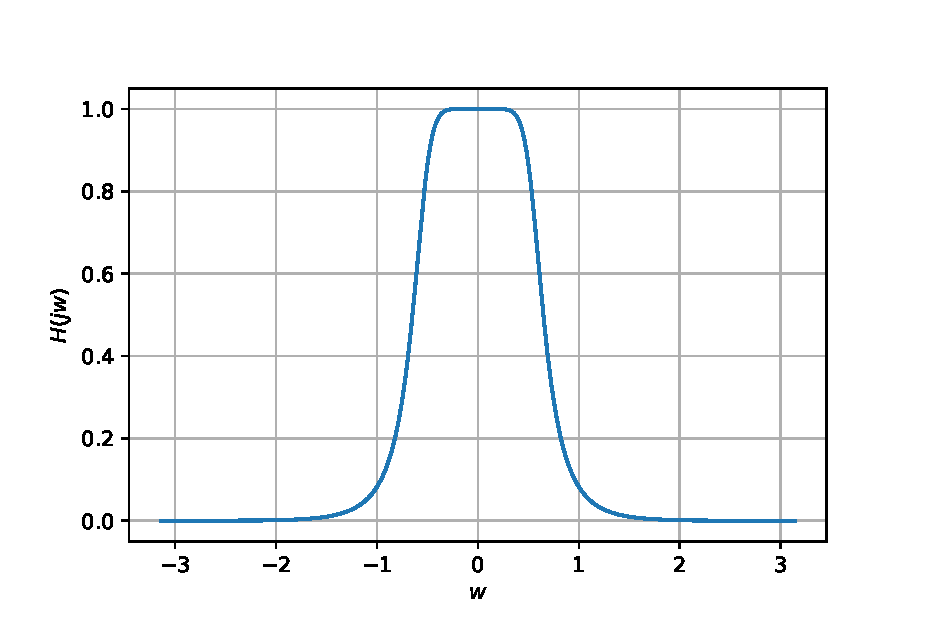
\includegraphics[width=\columnwidth]{H(jw)}
\caption{$\abs{H\brak{e^{\j w}}}$}
\label{fig:H(jw)}
\end{figure}
\end{enumerate}
\section{Impulse Response}
\begin{enumerate}[label=\thesection.\arabic*,ref=\thesection.\theenumi]
\item
From the difference equation eq. \ref{eq:diff_eqn}. Sketch h(n)
\label{prob:h(n)}
\\
\solution
When Input  = $\delta(k)$, Output = $h(k)$. \\We know that on shifting the input, the output will also shift.\\
Hence from eq.\ref{eq:iir_filter_gen}, 
by substituting $x(n-k) = \delta(n-k)$, then $y(n-k) = h(n-k)$ for all values of k.\\
Code for the plot in Fig.\ref{fig:h(n)}
\begin{lstlisting}
Codes/hn_plot.py
\end{lstlisting}
\begin{figure}[!ht]
\centering
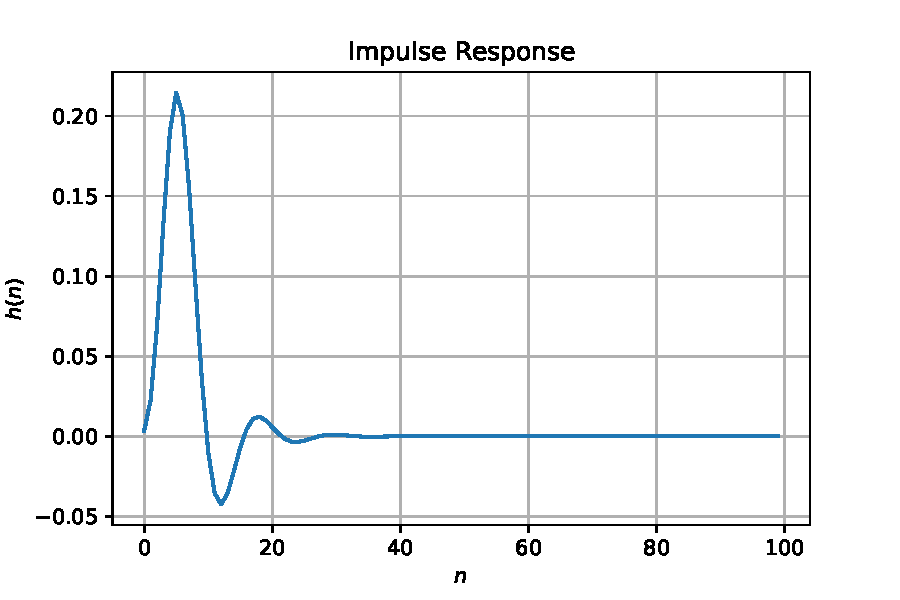
\includegraphics[width=\columnwidth]{h(n)}
\caption{$h(n)$}
\label{fig:h(n)}
\end{figure}
\item Check whether h(n) obtained is stable.
\\
\solution

We know that a system is stable if the following condition is satisfied. If the input is bounded, the output is bounded. This is known as BIBO stability.

From convolution formula,
\begin{equation}
\abs{y(n)} = \abs{\sum_{-\infty}^{\infty} h(k)x(n-k)}
\end{equation}
\begin{equation}
\abs{y(n)} \leq \sum_{-\infty}^{\infty} \abs{h(k)}\abs{x(n-k)}
\end{equation}
Let $B_{x}$ be the maximum value x(n-k) can take as the audio input is bounded, then
\begin{equation}
\abs{y(n)} \leq B_{x}\sum_{-\infty}^{\infty} \abs{h(k)}
\end{equation}
If
\begin{equation}
\sum_{-\infty}^{\infty} \abs{h(k)} < \infty
\end{equation}
Then
\begin{equation}
\abs{y(n)} \leq B_{y} < \infty
\end{equation}
Therefore to prove y(n) is bounded we need to prove h(n) is bounded.

\begin{equation}
\sum_{n=-\infty}^{n=-\infty} \abs{h(n)}<\infty
\end{equation}
The above equation can be re written as,
\begin{equation}
\sum_{n=-\infty}^{n=-\infty} \abs{h(n)z^{-n}}_{\abs{z}=1}<\infty
\end{equation}
\begin{equation}
\sum_{n=-\infty}^{n=-\infty} \abs{h(n)} \abs{z^{-n}}_{\abs{z}=1}<\infty
\end{equation}
From Triangle inequality,
\begin{equation}
\abs{\sum_{n=-\infty}^{n=-\infty} h(n)z^{-n}}_{\abs{z}=1}<\infty
\end{equation}
\begin{equation}
\implies \abs{H(n)}_{\abs{z}=1} < \infty
\end{equation}
From the equation \eqref{eq:freq_resp}
poles of the given transfer equation is:
\begin{equation}
\begin{split}
z(approx) = 0.69382 \pm 0.41i,
\\
 0.56617835 \pm 0.134423
\end{split}  
\end{equation}
From the above poles, we can see that that the ROC of the system is $\abs{z}>\sqrt{0.69382^{2}+0.41^{2}}$.
\begin{figure}[!ht]
\centering
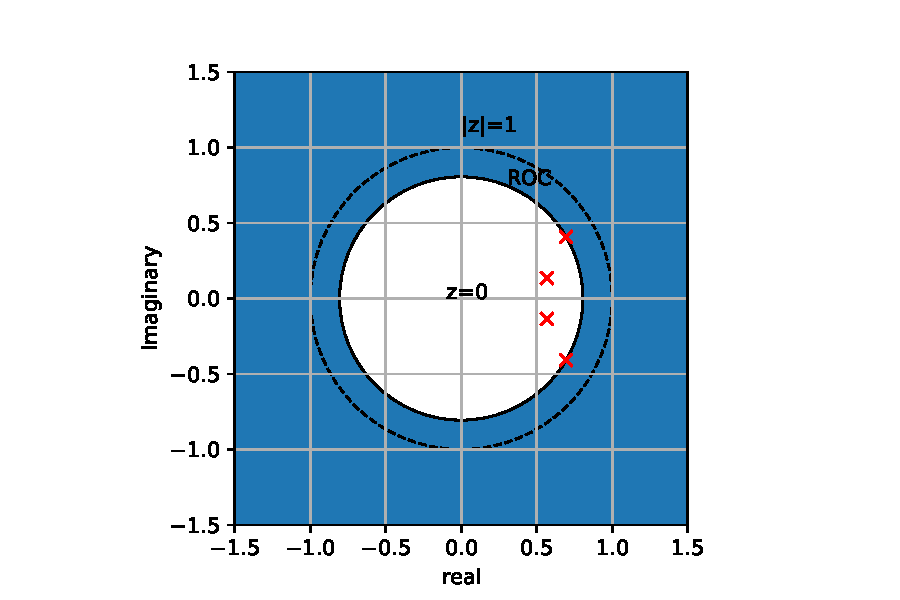
\includegraphics[width=\columnwidth]{ROC}
\caption{$X(k) and H(k)$}
\label{fig:xnhnfft}
\end{figure}
From the figure we can observe that ROC of the system includes unit circle $\abs{z}=1$.\\
The code for plotting the figure is:
\begin{lstlisting}
Codes/plot_roc.py
\end{lstlisting}
This implies that the given IIR filter is stable, because h(n) is absolutely summable. Hence y(n) is bounded, and stable.\\

\textbf{Verification from section 2}:-
Given bounded input x(n) (audio sample) and system difference equation \ref{eq:diff_eqn}
From \ref{fig:xnyn} we can see that the maximum value of x(n) is 0.839 and minimum value is greater than -0.94171.
For y(n) \ref{fig:xnyn} we observe the maximum value is 0.822256 and minimum value is -0.953761 and it tends to zero after a certain interval.
Therefore we can say that the system is BIBO stable.\\
\item Compute Filtered output using convolution formula using h(n) obtained in \ref{prob:h(n)}
%
\begin{equation}
\label{eq:convolution}
y(n) = x(n)*h(n) = \sum_{n=-\infty}^{\infty}x(k)h(n-k)
\end{equation}
\solution The following code plots Fig. \ref{fig:yn_conv}
%
\begin{lstlisting}
Codes/yn_convolution.py
\end{lstlisting}
\begin{figure}[!ht]
\centering
\includegraphics[width=\columnwidth]{yn_conv}
\caption{$y(n)$ from the definition of convolution}
\label{fig:yn_conv}
\end{figure}
The filtered sound signal through convolution from this method is found in
\begin{lstlisting}
Codes/Sound_convolution.wav
\end{lstlisting}
We can observe that the output obtained is same as y(n) obtained in Fig. \ref{fig:xnyn}
\end{enumerate}
\section{FFT and IFFT}
\begin{enumerate}[label=\thesection.\arabic*
,ref=\thesection.\theenumi]
\item Compute
\begin{align}
        X(k) \triangleq \sum_{n=0}^{N-1} x(n) e^{-j 2 \pi k n / N}, \quad k=0,1, \ldots, N-1
\end{align}
and $H(k)$ using h(n).
\\
\solution

DFT of a Input Signal $x(n)$ is 
\begin{align}
    X(k) \triangleq \sum_{n=0}^{N-1} x(n) e^{-j 2 \pi k n / N}, \quad k=0,1, \ldots, N-1
\end{align}
DFT of a Impulse Response $h(n)$ is 
\begin{align}
    H(k) \triangleq \sum_{n=0}^{N-1} h(n) e^{-j 2 \pi k n / N}, \quad k=0,1, \ldots, N-1
\end{align}
The following code plots FFT of $x(n)$,$y(n)$ and $h(n)$.
\begin{lstlisting}
    Codes/xn_hn_yn_fft.py
\end{lstlisting}
Magnitude and Phase plots obtained through above code is 
\begin{figure}[!ht]
\centering
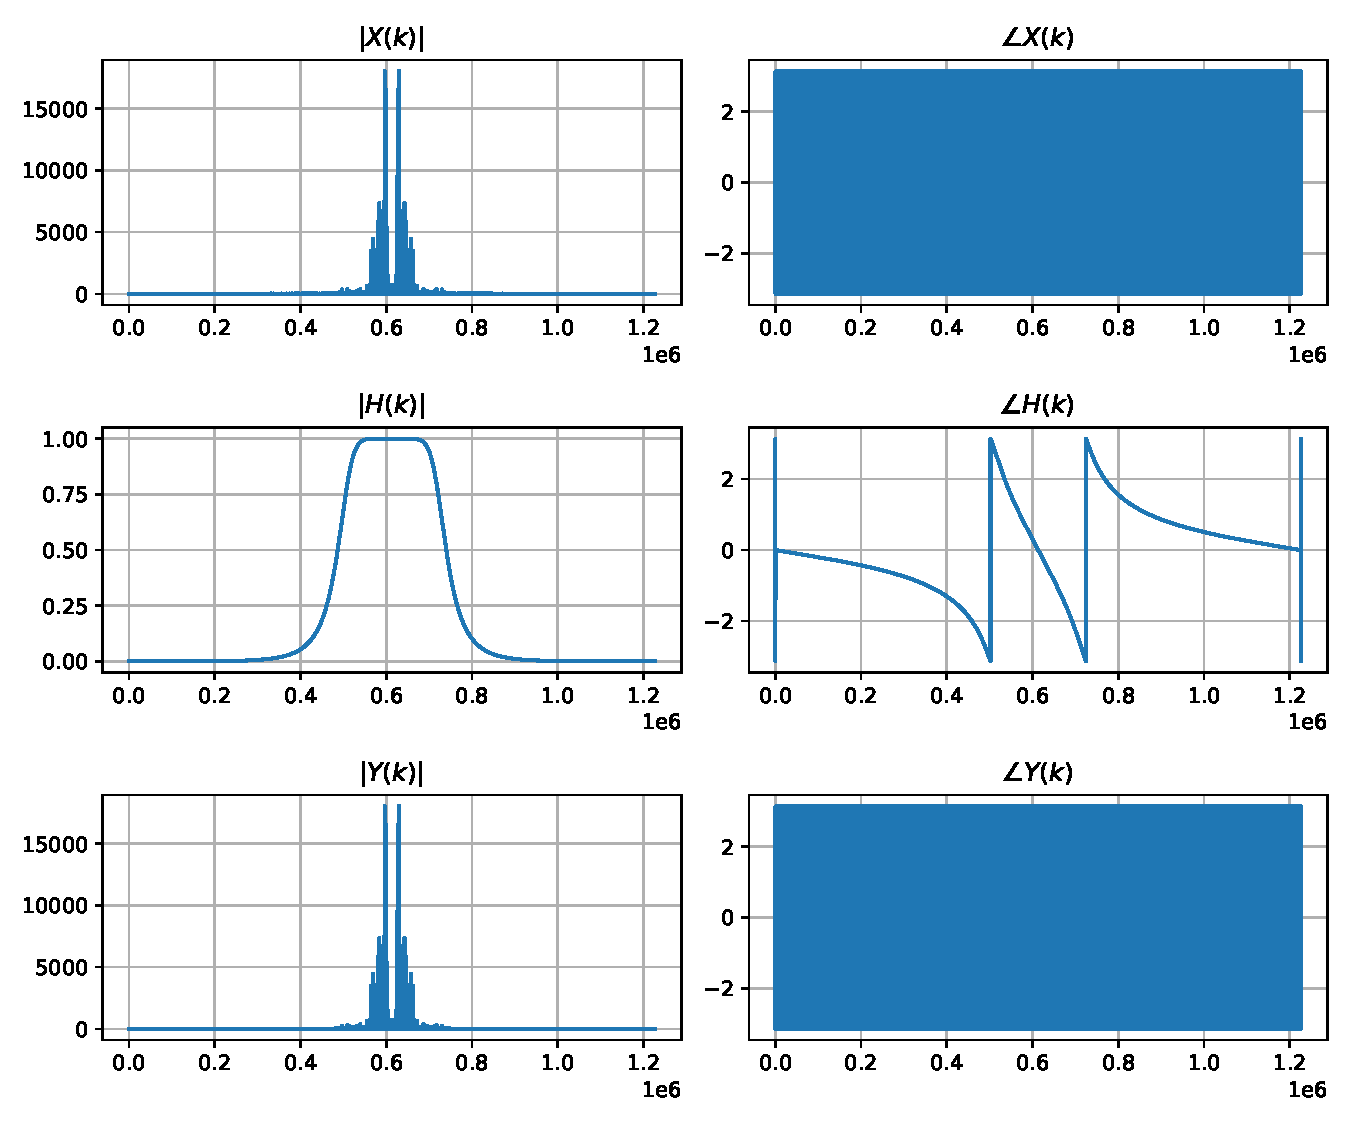
\includegraphics[width=\columnwidth]{xn_hn_yn_fft}
\caption{$X(k), H(k) and Y(k)$}
\label{fig:xnhnfft}
\end{figure}
\item From
\begin{equation}
Y(k) = X(k)H(k)
\end{equation}
Compute
\begin{equation}
y(n) \triangleq \sum_{k=0}^{N-1} Y(k) e^{j 2 \pi k n / N}, \quad n=0,1, \ldots, N-1
\end{equation}
\\
\solution
The following code plots Fig.\ref{fig:ynfft}
\begin{lstlisting}
    Codes/yn_fft.py
\end{lstlisting}
The IFFT of Y(k) gives the following plot.\\
\begin{figure}[!ht]
\centering
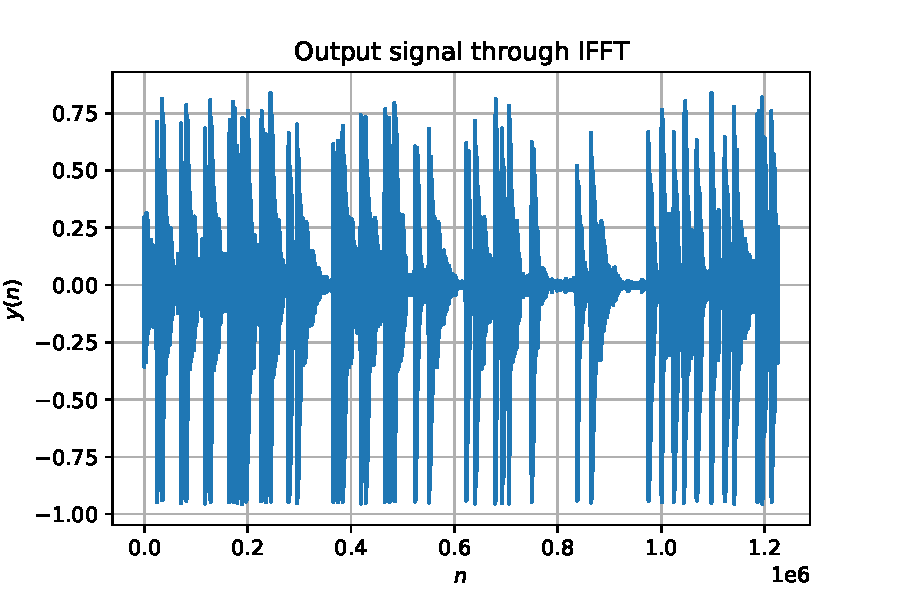
\includegraphics[width=\columnwidth]{yn_fft}
\caption{$y(n)$}
\label{fig:ynfft}
\end{figure}
The filtered sound signal from this method is found in
\begin{lstlisting}
Codes/Sound_fft.wav
\end{lstlisting}
This plot is same as that observed in Fig.\ref{fig:xnyn}
\end{enumerate}
\end{document}